\documentclass{VUMIFSlides}
\usepackage{times}
\usepackage[T1]{fontenc}
\usepackage{color}
\usepackage{verbatim}
\usepackage{graphicx}
\usepackage{fancyvrb}
\usepackage{bm}
\usepackage{amsfonts}
\usepackage{float}
\usepackage{hyperref}
\usepackage{adjustbox}
\usepackage{textpos} % FOR LOGO
\usepackage[english,lithuanian]{babel}
\usepackage{animate}
\usepackage{caption}

\usepackage{subfig}
\usepackage{pgfplots}
\usepackage{tikz}
\usetikzlibrary{quantikz2}
\pgfplotsset{compat=1.18} 

\hypersetup{
    pdfauthor=Pijus Petkevičius,
    linktoc=all,     %set to all if you want both sections and subsections linked
}

\title[Variacinio kvantinio tiesinių lygčių sistemų algoritmo pritaikymo  atraminių vektorių klasifikatoriui galimybių tyrimas]{Variacinio kvantinio tiesinių lygčių sistemų algoritmo pritaikymo  atraminių vektorių klasifikatoriui galimybių tyrimas}

\author[Pijus Petkevičius]{Pijus Petkevičius\\Programų sistemų 4 k. 1 gr.} 
\institute[VU MIF] 
{
Vilniaus Universitetas \\ 
\medskip
Pijus.Petkevicius@mif.stud.vu.lt
} 

\bibliography{bib}

% Let's get started
\begin{document}

\begin{frame}
  \maketitle
\end{frame}
\begin{frame}{Darbo tikslai ir uždaviniai}
    \textbf{Darbo tikslas}. Atlikti VQLS-SVM algoritmo tyrimą, siekiant išplėsti jo taikymą iki 10 kubitų.

    \textbf{Darbo uždaviniai.}
    \begin{itemize}
         \item Išanalizuoti VQLS-SVM algoritmą \cite{VQLS-SVM} straipsnyje, pritaikyti kodo optimizavimus, skirtus sumažinti algoritmo skaičiavimo trukmę.
    \item Atlikti tyrimus su skirtingomis duomenų aibėmis, palyginti klasikinio ir kvantinio atraminių vektorių klasifikatorių tikslumus.
    \item Atlikti įvairių gradientinių ir negradientinių optimizatorių bandymus, rasti efektyviausią optimizatorių problemos sprendimui.
    \item Išplėsti \cite{VQLS-SVM} straipsnyje pristatytą algoritmą iki 10 kubitų, siekiant padidinti apmokymo duomenų aibės dydį ir duomenų požymių skaičių. Toks išplėtimas leistų algoritmui efektyviai apdoroti sudėtingesnius duomenis ir padidinti klasifikavimo tikslumą.
    \item Pritaikyti Luko Hantzko straipsnyje \cite{TensorPauliDecomposition} pristatytą efektyvų tenzorinės Paulio bazės dekompozicijos algoritmą, kai kubitų skaičius pasiekia 10. 
    \item Ištirti ar Andrea Mari pristatytame straipsnyje nuoseklus variacinis kvantinis tiesinių lygčių sistemų algoritmas (\emph{angl. coherent variational quantum linear solver}) turi tam tikrų privalumų sprendžiant atraminių vektorių klasifikatoriaus problemą lyginant su VQLS algoritmu.\cite{CVQLS, VQLS}.
    \end{itemize}
\end{frame}
\begin{frame}{Atraminių vektorių klasifikatorius}
    \begin{columns}
        \begin{column}{0.5\textwidth}
            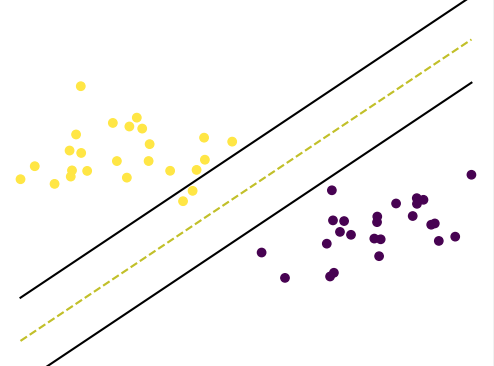
\includegraphics[scale=0.45]{img/svm.png}
        \end{column}
    
        \begin{column}{0.4\textwidth}
        Mažiausių kvadratų atraminių vektorių klasifikatoriaus (LSSVM) forma \cite{LSSVM}:
            \begin{equation}
                \begin{bmatrix}
                    0 & \vec{1}_N^T \\
                    \vec{1}_N & \Omega + \gamma^{-1} I_N
                \end{bmatrix} \cdot 
                \begin{bmatrix}
                    d \\
                    \vec{\theta}
                \end{bmatrix} = 
                \begin{bmatrix}
                    0 \\
                    \vec{y}    
                \end{bmatrix} \nonumber
            \end{equation}
            
            $\vec{1}_N = {\underbrace{[1;\ldots; 1]}_{N}}^T$, $\Omega = X^T X$ - tiesinė branduolio matrica, $\gamma$ - reguliavimo parametras, $d$ - poslinkio reikšmė, $\vec{\theta}$ - Lagranžo daugikliai , $\vec{y}$ - duomenų aibės klasių reikšmės.
        \end{column}
    \end{columns}
\end{frame}
\begin{frame}{\textit{Ansatz} grandinė}
    $$ V(\alpha)|0\rangle = \frac {|x\rangle }{\|x\|}, \quad\text{jei } \|x\| \ne 1\text{, kitu atveju - } V(\alpha)|0\rangle = |x\rangle$$
    \begin{center}
        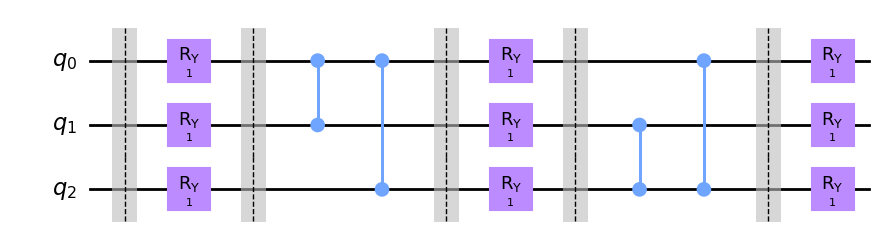
\includegraphics[scale=0.6]{img/ansatz.png}
    \end{center}
\end{frame}

\begin{frame}{\textit{Ansatz} grandinė}
    \begin{center}
        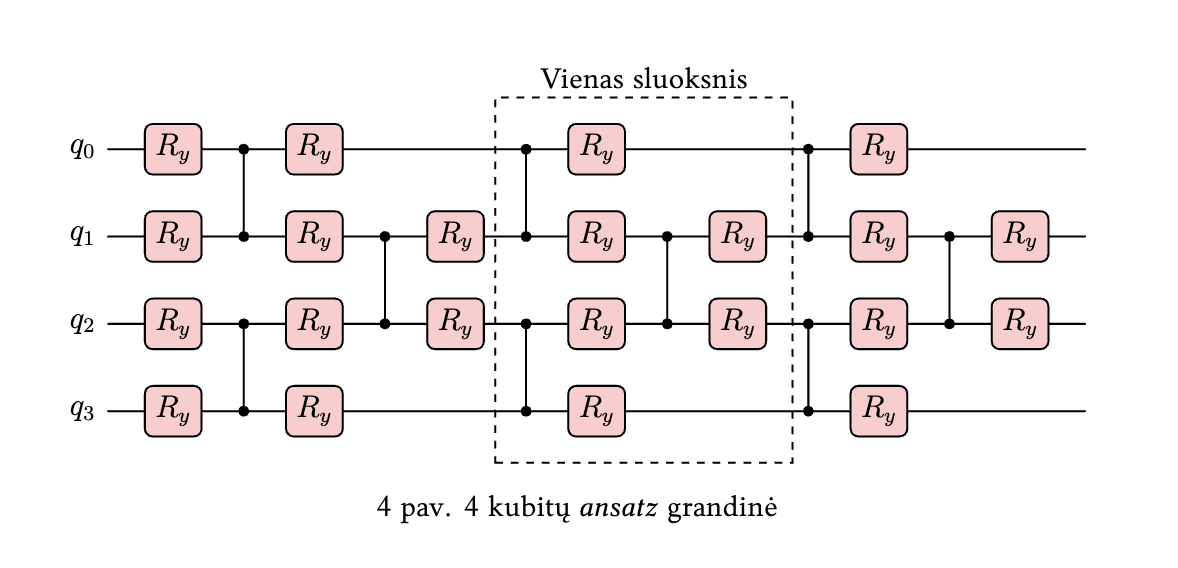
\includegraphics[scale=0.7]{img/ansatz4qubits.png}
    \end{center}
\end{frame}
\begin{frame}{Nuostolių funkcija}
    Sprendžiame performuluotą tiesinių lygčių sistemą:
    $$A |x\rangle \approx |b \rangle \equiv AV(\alpha)|0\rangle \approx |b\rangle$$

    Norint rasti geriausius $\alpha$ reikia minimizuoti nuostolių funkcijos reikšmę \cite{VQLS}:
    \begin{gather}
        H_P \ = \ \mathbb{I} \ - \ |b\rangle \langle b| \nonumber \\ 
        \hat{C}_P \ = \ \frac{\langle \psi | H_P | \psi \rangle \ } {\langle\psi|\psi\rangle} = \frac{\langle \psi | \psi \rangle}{\langle \psi | \psi \rangle} \ - \ \frac{\langle \psi |b\rangle \langle b | \psi \rangle}{\langle \psi | \psi \rangle} \ = \ 1 \ - \ \frac{\langle \psi |b\rangle \langle b | \psi \rangle}{\langle \psi | \psi \rangle} \ = \ 1 \ - \ \frac{|\langle b | \psi \rangle|^2}{\langle \psi | \psi \rangle} \nonumber
     \end{gather}
\end{frame}

\begin{frame}{$\langle \psi|\psi\rangle$ apskaičiavimas}
    \begin{gather}
        \langle \psi | \psi \rangle \ =  \langle 0 | V(\alpha)^{\dagger} A^{\dagger} A V(\alpha) |0\rangle \ = \ \langle 0 | V(\alpha)^{\dagger} \Big( \displaystyle\sum_{m} c_m \ A_m \Big)^{\dagger} \Big( \displaystyle\sum_{n} c_n \ A_n \Big) V(\alpha) |0\rangle = \nonumber \\ 
        = \sum_{m} \sum_{n} \overline{c_{m}} c_{n} \langle 0 | V(\alpha)^\dag A_{m}^\dag A_{n} V(\alpha)|0\rangle \nonumber
    \end{gather}
    \begin{center}
        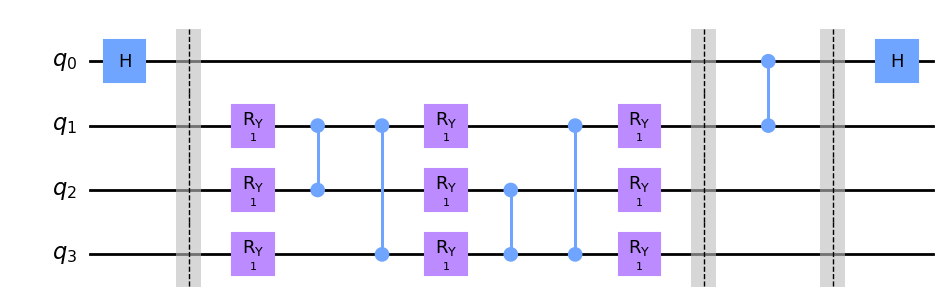
\includegraphics[scale=0.6]{img/hadamardTest.png}
    \end{center}
\end{frame}

\begin{frame}{Taisyklės}
    \begin{center}
        \includegraphics[scale=0.3]{img/rules.png}
    \end{center}
\end{frame}

\begin{frame}{$|\langle b|\psi \rangle|^2$ apskaičiavimas}
    \begin{gather}
         |\langle b | \psi \rangle|^2 \ = \ |\langle b | A V(\alpha) | 0 \rangle|^2 \ = \ |\langle 0 | U^{\dagger} A V(\alpha) | 0 \rangle|^2 \ = \ \langle 0 | U^{\dagger} A V(\alpha) | 0 \rangle \langle 0 | V(\alpha)^{\dagger} A^{\dagger} U |0\rangle = \nonumber \\
        = \ \displaystyle\sum_{m} \displaystyle\sum_{n} \overline{c_m} c_n \langle 0 | U^{\dagger} A_n V(\alpha) | 0 \rangle \langle 0 | V(\alpha)^{\dagger} A_m^{\dagger} U |0\rangle \nonumber
    \end{gather}
     \begin{center}
        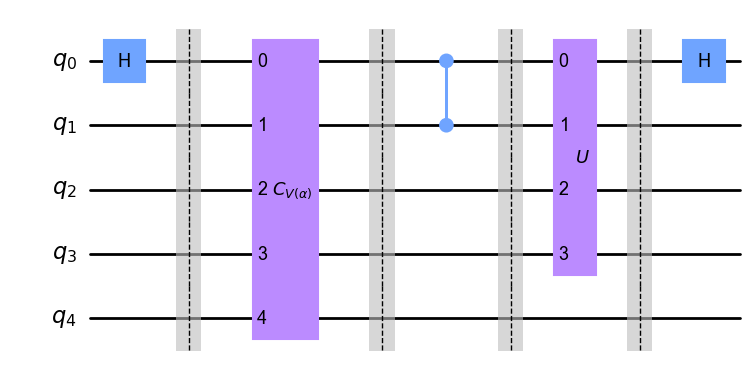
\includegraphics[scale=0.55]{img/specialHadamardTest.png}
    \end{center}
\end{frame}

\begin{frame}{VQLS-SVM algoritmas}
    \begin{center}
        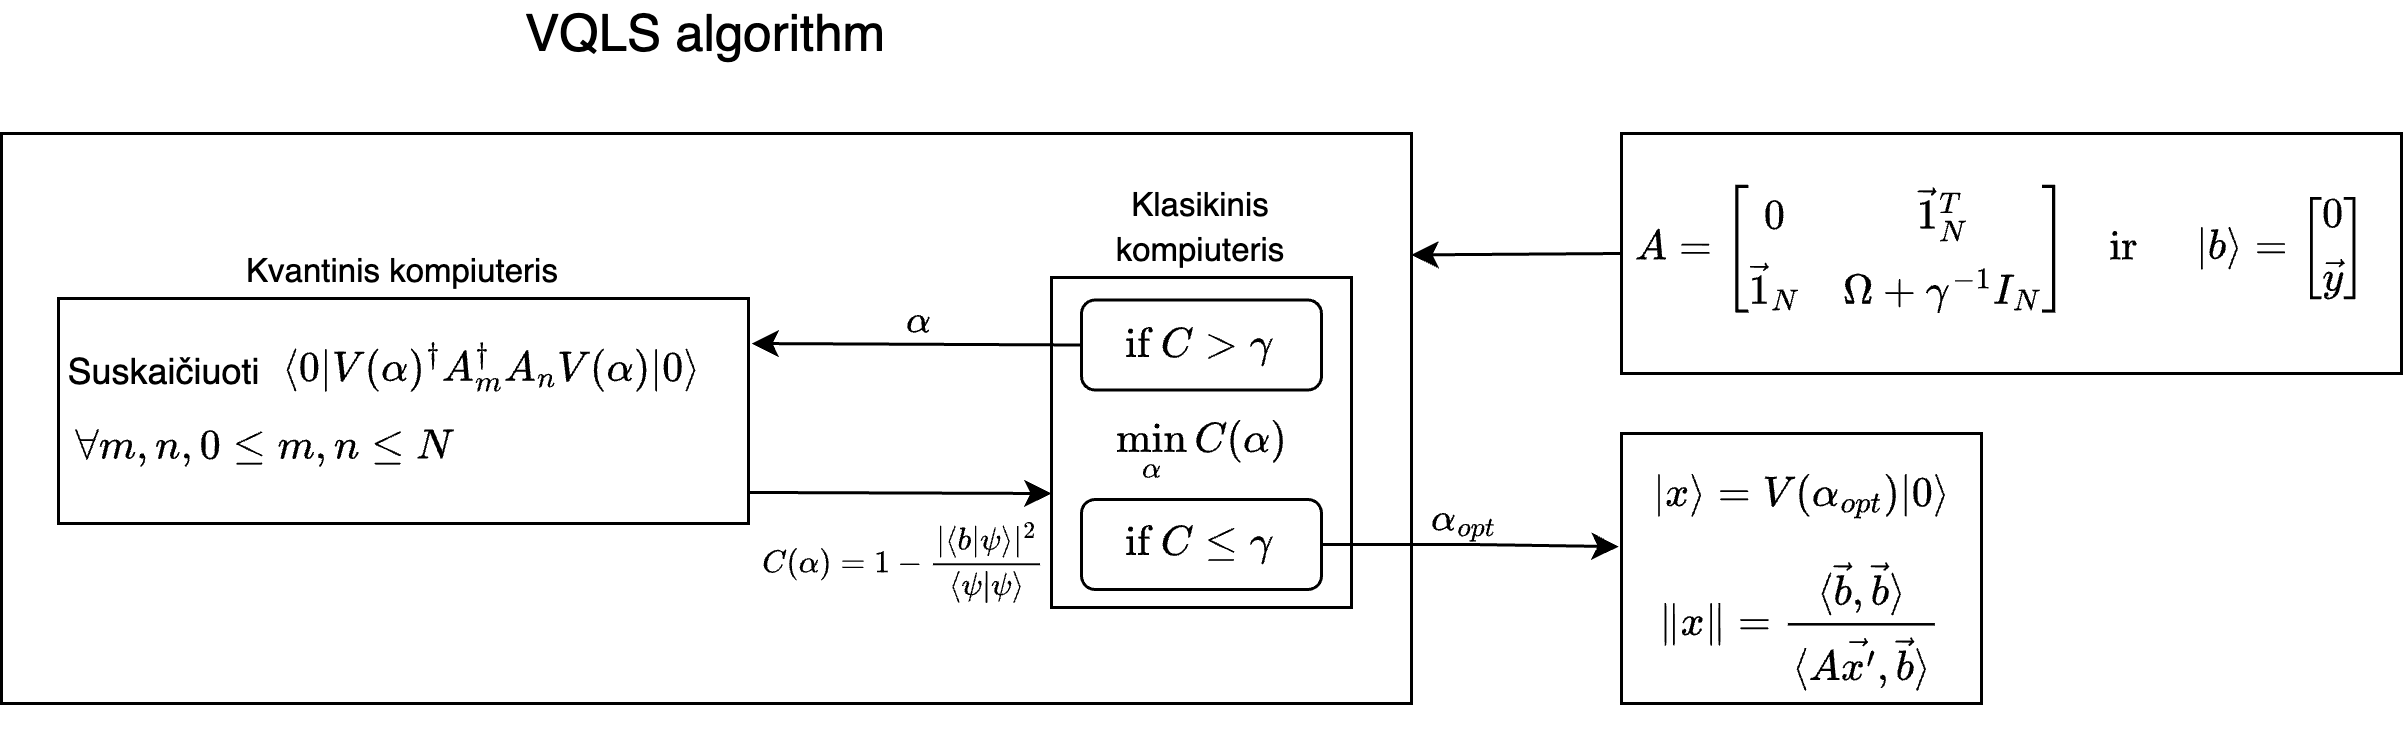
\includegraphics[scale=0.18]{img/VQLS.drawio.png}
    \end{center}
\end{frame}
\begin{frame}{Duomenų paruošimas}
    \begin{itemize}
        \item VQLS-SVM ir SVM algoritmų mokymui iš irisų duomenų aibės pašalinta Iris virginica duomenys ir atsitiktinai parinkti 7 įrašai. Iris Setosa duomenų klasė pakeista į $-1$, Iris Versicolour į $1$.
        \item Krūties auglių duomenų rinkinio atsitiktinai paimti 7 įrašai. Benign duomenų klasė pervadinta į $-1$, malignant į $1$.
        \item Sukonstruojama LSSVM esanti matrica, naudojantis duomenimis. Duomenų klasės atitinkamai užkoduojamos į $\left[0\  \vec{y}\right]^T$. Paruošta matrica išskaidoma į unitarines, su koeficientais:
        \begin{gather}
            A = \sum_{l=0}^N c_l A_l, \quad c\in \mathbb{C} \nonumber\\
            A_l \in \{I,X,Y,Z\}^{\otimes N}\nonumber
        \end{gather}    
            
    \end{itemize}
\end{frame}

\begin{frame}{Irisų duomenų rinkinio mokymas}
    \begin{center}
        % \begin{tikzpicture}
        %     \begin{axis}[
        %         ticklabel style={font=\small,fill=none},
        %         xticklabel style={yshift=-10pt},
        %         yticklabel style={xshift=-10pt},
        %         cycle list name=auto,
        %         xlabel={Iteracijų skaičius},
        %         ylabel={Nuostolių funkcijos reikšmė},
        %         xmin=0, xmax=115,
        %         ymin=0, ymax=1, ytick={0.1,0.2,0.3,0.4,0.5,0.6,0.7,0.8,0.9,1},
        %         legend pos=outer north east,
        %         ymajorgrids=true,
        %         grid style=dashed,
        %         % legend entries={irisai},
        %         width=10cm,
        %         height=7cm
        %         ]
                
        %        \addplot table[x=Iteration, y=IrisCostFunction, col sep=comma] {Data/costCOBYLAIris.csv};
        %     \end{axis}
        % \end{tikzpicture}

            \begin{tikzpicture}
                \begin{axis}[
                    cycle list name=auto,
                    xlabel={Iteracijų skaičius},
                    ylabel={Nuostolių funkcijos reikšmė},
                    xmin=0, xmax=116,
                    ymin=0, ymax=1, ytick={0.1,0.2,0.3,0.4,0.5,0.6,0.7,0.8,0.9,1},
                    legend pos= north east,
                    ymajorgrids=true,
                    grid style=dashed,
                    % legend entries={irisai},
                    width=10cm,
                    height=7cm
                    ]
                    \addplot table[x=Iteration, y=iris, col sep=comma] {Data/costDatasetiris.csv};
                    \addplot table[x=Iteration, y=iris, col sep=comma] {Data/costDatasetirisOneVsAll.csv};
               \legend{VQLS-SVM išmetant vieną klasę, VQLS-SVM 1 vs all metodu}  
                \end{axis}
            \end{tikzpicture}
    \end{center}
\end{frame}

\begin{frame}{VQLS-SVM ir SVM klasifikavimo tikslumas}
    \begin{center}
            \begin{tikzpicture}  
                \begin{axis}  
                [  
                    ybar=10pt, % ybar command displays the graph in horizontal form, while the xbar command displays the graph in vertical form.  
                    bar width=1cm,
                    enlargelimits=0.2,% these limits are used to shrink or expand the graph. The lesser the limit, the higher the graph will expand or grow. The greater the limit, the more graph will shrink.   
                    legend style={at={(0.4,-0.25)}, % these are the measures of the bottom row containing surplus (wheat, Tea, rice), where -0.25 is the gap between the bottom row and the graph.   
                    anchor=north,legend columns=-1},     
                      % here, north is the position of the bottom legend row. You can specify the east, west, or south direction to shift the location.   
                    ylabel={Algoritmo klasifikavimo tikslumas}, % there should be no line gap between the rows here. Otherwise, latex will show an error.  
                    symbolic x coords={Iris Setosa, Irisų Virginica, Iris Versicolour},  
                    xtick=data,  
                    nodes near coords,  
                    nodes near coords align={vertical},  
                    width=10cm,
                    height=7cm
                    ]  
                \addplot coordinates {(Iris Setosa,86.50) (Irisų Virginica, 61.96) (Iris Versicolour, 53.29) }; % these are the measures of a particular bar graph. The tick marks of the y-axis will be adjusted automatically according to the data values entered in the coordinates.  
                \addplot coordinates {(Iris Setosa, 99.51) (Irisų Virginica,79.86) (Iris Versicolour, 64.83)};  
                \legend{VQLS-SVM, SVM}  
                \end{axis}  
            \end{tikzpicture}   
    \end{center}
\end{frame}


\begin{frame}{VQLS-SVM ir SVM klasifikavimo tikslumas}
    \begin{center}
      \begin{tikzpicture}  
                \begin{axis}  
                [  
                    ybar=10pt, % ybar command displays the graph in horizontal form, while the xbar command displays the graph in vertical form.  
                    bar width=1cm,
                    enlargelimits=0.2,% these limits are used to shrink or expand the graph. The lesser the limit, the higher the graph will expand or grow. The greater the limit, the more graph will shrink.   
                    legend style={at={(0.4,-0.25)}, % these are the measures of the bottom row containing surplus (wheat, Tea, rice), where -0.25 is the gap between the bottom row and the graph.   
                    anchor=north,legend columns=-1},     
                      % here, north is the position of the bottom legend row. You can specify the east, west, or south direction to shift the location.   
                    ylabel={Algoritmo klasifikavimo tikslumas}, % there should be no line gap between the rows here. Otherwise, latex will show an error.  
                    symbolic x coords={Irisų duomenys, Irisų duomenys 1 vs all, Krūties auglių duomenys},  
                    xtick=data,  
                    nodes near coords,  
                    nodes near coords align={vertical},  
                    width=15cm,
                    height=8cm
                    ]  
                \addplot coordinates {(Irisų duomenys,92.25806451612902) (Irisų duomenys 1 vs all, 66.43356643356644) (Krūties auglių duomenys, 55.4270462633452) }; % these are the measures of a particular bar graph. The tick marks of the y-axis will be adjusted automatically according to the data values entered in the coordinates.  
                \addplot coordinates {(Irisų duomenys, 100) (Irisų duomenys 1 vs all,81.74825174825175) (Krūties auglių duomenys, 90.7473309608541)};  
                \legend{VQLS-SVM, SVM}  
                 
                \end{axis}  
            \end{tikzpicture}    
    \end{center}
\end{frame}
\begin{frame}{Frame Title}
    \begin{center}

     \begin{tikzpicture}
                \begin{axis}[
                  xmin = 7, xmax = 31, xtick={7,19,31},
                  xticklabels={7, 15, 31},
                  ymin = 50, ymax = 100, % leave as is 
                  axis x line*=top,
                  hide y axis,
                  xlabel={Apmokymo aibės dydis},
                  xlabel near ticks,
                  width=10cm,
                  height=4cm
                ]
                \end{axis}
                \begin{axis}[
                    cycle list name=auto,
                    xlabel={Kubitų skaičius},
                    ylabel={Klasifikavimo tikslumas},
                    xmin=3, xmax=5, xtick={3,4,5},
                    ymin=50, ymax=100, ytick={50,60,70,80,90,100},
                    legend pos= south east,
                    ymajorgrids=true,
                    grid style=dashed,
                    width=10cm,
                    height=4cm
                    ]
               
                    \addplot table[x=Kubitai, y=Tikslumas, col sep=comma] {Data/qubitsBreast.csv};
                   \addplot table[x=Kubitai, y=TikslumasSvm, col sep=comma] {Data/qubitsBreast.csv};
                   \legend{VQLS-SVM, SVM}
                \end{axis}
            \end{tikzpicture}
            \end{center}
\end{frame}
\begin{frame}{Frame Title}
    \begin{center}
                    \begin{tabular}{@{}c@{}}
                \begin{tikzpicture}
                    \begin{axis}[
                      xmin = 7, xmax = 31, xtick={7,19,31},
                      xticklabels={7, 15, 31},
                      ymin = 90, ymax = 100, % leave as is 
                      axis x line*=top,
                      hide y axis,
                      xlabel={Apmokymo aibės dydis},
                      xlabel near ticks,
                      width=10cm,
                      height=4cm
                    ]
                    \end{axis}
                    \begin{axis}[
                        cycle list name=auto,
                        xlabel={Kubitų skaičius},
                        ylabel={Klasifikavimo tikslumas},
                        xmin=3, xmax=5, xtick={3,4,5},
                        ymin=90, ymax=100, ytick={90,92,94,96,98,100},
                        legend pos=south east,
                        ymajorgrids=true,
                        grid style=dashed,
                        width=10cm,
                        height=4cm
                        ]
                   
                        \addplot table[x=Kubitai, y=Tikslumas, col sep=comma] {Data/qubitsIris.csv};
                        \addplot table[x=Kubitai, y=TikslumasSVM, col sep=comma] {Data/qubitsIris.csv};
                       \legend{VQLS-SVM, SVM}  
                    \end{axis}
                \end{tikzpicture} \\
                % \caption{test}
                \small (a) Išmetus Iris Virginica duomenų klasės elementus \\
                \label{fig:subfigOneVSALL1}
            \end{tabular}
            \begin{tabular}{@{}c@{}}
                \begin{tikzpicture}
                     \begin{axis}[
                      xmin = 7, xmax = 31, xtick={7,19,31},
                      xticklabels={7, 15, 31},
                      ymin = 90, ymax = 100, % leave as is 
                      axis x line*=top,
                      hide y axis,
                      xlabel={Apmokymo aibės dydis},
                      xlabel near ticks,
                      width=10cm,
                      height=4cm
                    ]
                    \end{axis}
                    \begin{axis}[
                        cycle list name=auto,
                        xlabel={Kubitų skaičius},
                        ylabel={Klasifikavimo tikslumas},
                        xmin=3, xmax=5, xtick={3,4,5},
                        ymin=50, ymax=100, ytick={50,60,70,80,90,100},
                        legend pos= south east,
                        ymajorgrids=true,
                        grid style=dashed,
                        width=10cm,
                        height=4cm
                        ]
                        \addplot table[x=Kubitai, y=Tikslumas, col sep=comma] {Data/qubitsIris1VSAll.csv};
                        \addplot table[x=Kubitai, y=TikslumasSVM, col sep=comma] {Data/qubitsIris1VSAll.csv};
                       \legend{VQLS-SVM, SVM}  
                    \end{axis}
                \end{tikzpicture} \\
                \small (b) Naudojantis vienas prieš visus (\emph{angl. one vs all}) metodu
                \label{fig:subfigOneVSALL2}
            \end{tabular}
    \end{center}
\end{frame}
\begin{frame}{Optimizatorių funkcijos}
    \begin{center}
        \begin{tikzpicture}
            \begin{axis}[
                ticklabel style={font=\small,fill=none},
                xticklabel style={yshift=-10pt},
                yticklabel style={xshift=-10pt},
                cycle multi list={%
                    color list\nextlist
                    [1 of]mark list
                },
                xlabel={Iteracijų skaičius},
                ylabel={Nuostolių funkcijos reikšmė},
                xmin=0, xmax=140,
                ymin=0, ymax=1, ytick={0.1,0.2,0.3,0.4,0.5,0.6,0.7,0.8,0.9,1},
                legend pos=north east,
                ymajorgrids=true,
                grid style=dashed,
                legend entries={SLSQP,COBYLA,trust-constr},
                width=10cm,
                height=7cm
                ]
                \addplot
                table[x=Iteration, y=SLSQP, col sep=comma] {Data/costOptimizers.csv};       
                \addplot
                table[x=Iteration, y=COBYLA, col sep=comma] {Data/costOptimizers.csv};
                \addplot [
                    color=green,
                    mark=triangle,
                ]
                table[x=Iteration, y=trust-constr, col sep=comma] {Data/costOptimizers.csv};
            \end{axis}
        \end{tikzpicture} \\
    \end{center}
\end{frame}
\begin{frame}{Optimizatorių funkcijos}
    \begin{center}
        \begin{tikzpicture}
            \begin{axis}[
                ticklabel style={font=\small,fill=none},
                xticklabel style={yshift=-10pt},
                yticklabel style={xshift=-10pt},
                cycle multi list={%
                    color list\nextlist
                    [1 of]mark list
                },
                xlabel={Iteracijų skaičius},
                ylabel={Nuostolių funkcijos reikšmė},
                xmin=0, xmax=140,
                ymin=0, ymax=1, ytick={0.1,0.2,0.3,0.4,0.5,0.6,0.7,0.8,0.9,1},
                legend pos=north east,
                ymajorgrids=true,
                grid style=dashed,
                legend entries={BFGS,L-BFGS-B,trust-constr},
                width=10cm,
                height=7cm
                ]
                \addplot [
                    color=violet,
                    mark=triangle,
                ]
                table[x=Iteration, y=BFGS, col sep=comma] {Data/costOptimizers.csv};
                \addplot [
                    color=orange,
                    mark=triangle,
                ]
                table[x=Iteration, y=L-BFGS-B, col sep=comma] {Data/costOptimizers.csv};
                \addplot [
                    color=green,
                    mark=triangle,
                ]
                table[x=Iteration, y=trust-constr, col sep=comma] {Data/costOptimizers.csv};
            \end{axis}
        \end{tikzpicture} \\
    \end{center}
\end{frame}

\begin{frame}{Frame Title}
    \begin{center}
                        \begin{tikzpicture}
                    \begin{axis}[
                        cycle multi list={%
                            color list\nextlist
                            [1 of]mark list
                        },
                        xlabel={Iteracijų skaičius},
                        ylabel={Nuostolių funkcijos reikšmė},
                        xmin=0, xmax=200,
                        ymin=0, ymax=1, ytick={0.1,0.2,0.3,0.4,0.5,0.6,0.7,0.8,0.9,1},
                        legend pos=north east,
                        ymajorgrids=true,
                        grid style=dashed,
                        legend entries={$\alpha=0.1$, $\alpha=0.5$, $\alpha=0.75$, $\alpha=0.9$},
                        width=16cm,
                        height=8cm
                        ]
                        \addplot
                        table[x=Iteration, y=ADAM_0.1, col sep=comma] {Data/costOptimizersGradient.csv};       
                        \addplot
                        table[x=Iteration, y=ADAM_0.5, col sep=comma] {Data/costOptimizersGradient.csv};

                        \addplot [
                            color=violet,
                            mark=triangle,
                        ]
                        table[x=Iteration, y=ADAM_0.75, col sep=comma] {Data/costOptimizersGradient2.csv};

                        \addplot [
                            color=green,
                            mark=triangle,
                        ]
                        table[x=Iteration, y=ADAM_0.9, col sep=comma] {Data/costOptimizersGradient2.csv};
                    \end{axis}
                \end{tikzpicture}
    \end{center}
\end{frame}

\begin{frame}{Frame Title}
    \begin{center}
                        \begin{tikzpicture}
                    \begin{axis}[
                        cycle multi list={%
                            color list\nextlist
                            [1 of]mark list
                        },
                        xlabel={Iteracijų skaičius},
                        ylabel={Nuostolių funkcijos reikšmė},
                        xmin=0, xmax=200,
                        ymin=0, ymax=1, ytick={0.1,0.2,0.3,0.4,0.5,0.6,0.7,0.8,0.9,1},
                        legend pos=south west,
                        ymajorgrids=true,
                        grid style=dashed,
                        legend entries={$\alpha=0.5$, $\alpha=0.6$, $\alpha=0.7$, $\alpha=0.8$, $\alpha=0.9$ },
                        width=16cm,
                        height=8cm
                        ]
                        \addplot 
                        table[x=Iteration, y=GD_0.5, col sep=comma] {Data/costOptimizersGradient.csv};
                         \addplot
                        table[x=Iteration, y=GD_0.6, col sep=comma] {Data/costOptimizersGradient2.csv};    
                         \addplot
                         [
                            color=orange,
                            mark=triangle,
                        ]
                        table[x=Iteration, y=GD_0.7, col sep=comma] {Data/costOptimizersGradient2.csv};    
                         \addplot
                         [
                            color=green,
                            mark=triangle,
                        ]
                        table[x=Iteration, y=GD_0.8, col sep=comma] {Data/costOptimizersGradient2.csv};    
                         \addplot
                            [
                            color=violet,
                            mark=triangle,
                        ]
                        table[x=Iteration, y=GD_0.9, col sep=comma] {Data/costOptimizersGradient2.csv};    
                    \end{axis}
                \end{tikzpicture}
    \end{center}
\end{frame}

\begin{frame}{Frame Title}
    \begin{center}
        \begin{tikzpicture}
                    \begin{axis}[
                        cycle multi list={%
                            color list\nextlist
                            [1 of]mark list
                        },
                        xlabel={Iteracijų skaičius},
                        ylabel={Nuostolių funkcijos reikšmė},
                        xmin=0, xmax=140,
                        ymin=0, ymax=1, ytick={0.1,0.2,0.3,0.4,0.5,0.6,0.7,0.8,0.9,1},
                        legend pos=north east,
                        ymajorgrids=true,
                        grid style=dashed,
                        legend entries={ADAM $\alpha = 0.5$, COBYLA,Gradient descend $\alpha = 0.9$,SLSQP},
                        width=16cm,
                        height=8cm
                        ]
                        \addplot
                        table[x=Iteration, y=ADAM_0.5, col sep=comma] {Data/costOptimizersGradient.csv};   
                        \addplot
                        table[x=Iteration, y=COBYLA, col sep=comma] {Data/costOptimizers.csv};
                        \addplot [
                            color=violet,
                            mark=triangle,
                        ]
                        table[x=Iteration, y=GD_0.9, col sep=comma] {Data/costOptimizersGradient2.csv};
                        \addplot
                        [
                            color=green,
                            mark=triangle,
                        ]
                        table[x=Iteration, y=SLSQP, col sep=comma] {Data/costOptimizers.csv};     
                    \end{axis}
                \end{tikzpicture} 
    \end{center}
\end{frame}
\section{Išvados}

\begin{frame}{Išvados}
    % \begin{enumerate}
    %     \item VQLS-SVM algoritmas tiksliai klasifikuoja testavimo duomenų rinkinį, kai apmokymo duomenų aibė turi tik 7 įrašus. Kvantinio atraminių vektorių klasifikatoriaus algoritmo tikslumas yra šiek tiek mažesnis lyginant su klasikiniu algoritmu. Gautas vektorius $x$ nėra tikslus sprendinys, kas turi įtakos klasifikavimo tikslumui. 
    %     \item Atlikus VQLS-SVM algoritmo tyrimą, buvo pastebėta, kad požymių skaičiui esant didesniam negu apmokymo duomenų aibė, klasifikavimo tikslumas yra mažesnis lyginant su duomenų rinkiniu, kurio požymių skaičius mažesnis už apmokymo aibę. 
    %     \item \textit{COBYLA} optimizatorius, iš tirtų išvestinių nereikalaujančių optimizatorių, greičiausiai pasiekė nuostolių funkcijos minimalią reikšmę. \textit{SQLSP} optimizavimo funkcija gali būti efektyvi optimizavimo funkcijos alternatyva, kai reikalingas didesnis skaičiavimų stabilumas, nes naudojant šį algoritmą, nuostolių funkcijos reikšmė didėjant iteracijų skaičiui, nedidėjo.
    % \end{enumerate}
\end{frame}

% \begin{frame}
%     %\frametitle{A first slide}
%     \begin{center}
%         \Huge Thank you for your attention!
%     \end{center}
% \end{frame}

\section{Benefits}

 \begin{frame}[c]{Ateities darbai}
        % \begin{enumerate}
        %     \item Išplėsti \textit{ansatz} grandinę iki 10 kubitų, siekiant padidinti apmokymo duomenų aibės dydį ir duomenų požymių skaičių. Toks išplėtimas leistų algoritmui efektyviai apdoroti sudėtingesnius duomenis ir padidinti klasifikavimo tikslumą.
        %     \item Didinant \textit{ansatz} grandinę iki 10 kubitų galime susidurti, kad matricos išskaidymas naudojantis  Qiskit pristatyta SparsePauliOP funkcija, truks ženkliai ilgiau, lyginant su $3$ kubitų atveju. Lukas Hantzko straipsnyje pristatytas efektyvus tenzorinės Paulio bazės dekompozicijos algoritmas, kai kubitų skaičius pasiekia 10 \cite{TensorPauliDecomposition}. 
    
        %     \item Pritaikyti gradientinio nusileidimo optimizavimo algoritmus (ADAM,SPSA) ir atlikti tyrimus.
        %     \item Ištirti ar Andrea Mari pristatytame straipsnyje nuoseklus variacinis kvantinis tiesinių lygčių sistemų algoritmas (\emph{angl. coherent variational quantum linear solver}) turi tam tikrų privalumų sprendžiant atraminių vektorių klasifikatoriaus problemą \cite{CVQLS}.
        % \end{enumerate} 
\end{frame}

\end{document}
